\documentclass[12pt]{article}
\usepackage[utf8]{inputenc}
\usepackage{lmodern}
\usepackage[margin=2.5cm]{geometry}
\usepackage{graphicx}


\title{Práctica 1}
\author{Fernando Cruz Pineda \\ Alexys Gómez Elizalde \\ Moisés Corpus García}
\date{}

\begin{document}
\maketitle

\section*{Ejercicios}

\begin{enumerate}
    \item Lee lo siguiente \texttt{https://www.evanjones.ca/software/threading-linus-msg.html} y comparte en máximo 4 líneas de computadora a qué se refiere Linus Torvalds con un contexto de ejecución y cómo se relaciona con la definición en la sección 1 de esta práctica.

    Linus explica que un contexto de ejecución es todo lo que necesita un hilo o proceso para ejecutarse: su stack, registros y estado. Se relaciona con la definición de la práctica porque ahí se habla de los hilos como “un flujo de control con su propio contexto de ejecución” que permite correr varias tareas en paralelo
    
    \item ¿Cuántos hilos tiene disponibles tu computadora? \\
      Ejecuta \texttt{Runtime.getRuntime().availableProcessors()}, si son más de uno en el equipo escriban el de cada uno.

      Número de hilos de Fernando Cruz: 8

      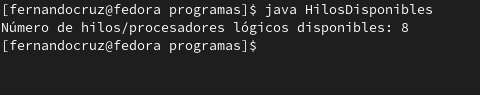
\includegraphics[]{Fer.png}

      Número de hilos de Alexys Gómez:12

      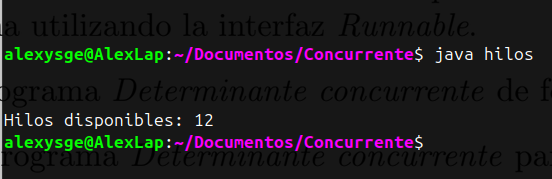
\includegraphics[]{1Alexys.png}

<<<<<<< HEAD
=======
      Número de hilos de Moisés Corpus: 16

      
\includegraphics[]{ProcesadoresLogicos_Moises_Corpus_Garcia.png}
>>>>>>> 6bd59094f9a3f04e6f6eb8d05cf62b2b6e89bf9e

    \item Revisa el programa Determinante Concurrente y responde ¿Cuánto tiempo tarda en ejecutarse?

      Tiempo en equipo de Fernando: 1755939 ns

      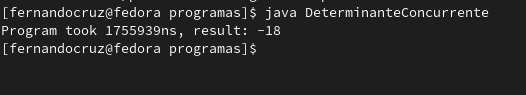
\includegraphics[]{Fer2.png}

      Tiempo en equipo de Alexys: 2000939 ns

      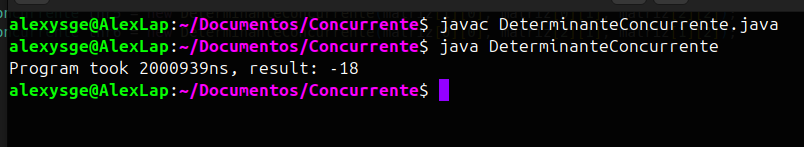
\includegraphics[]{2Alexys.png}

      Tiempo en equipo de Moises: 570900 ns

      
\includegraphics[]{DeterminanteConcurrente_Moises_Corpus_Garcia.png}

      
    \item El programa Determinante Concurrente está implementado extendiendo la clase Thread. Implementa el programa utilizando la interfaz Runnable.

      Programa en programas/DeterminanteConcurrenteRunnable.java

      Este programa tiene la misma lógica que el que extiende de la clase Thread, pues son 6 hilos que usando la regla de Sarrus calcula el determinante. La diferencia principal es que la lógica del cálculo se separa de la gestión de los hilos.
      
    \item Implementa el programa Determinante Concurrente de forma secuencial.
      
      Programa en programas/DeterminanteSecuencial.java

      Este programa calcula el determinante de una matriz 3x3 de forma secuencial, 
aplicando directamente la regla de Sarrus.  No utiliza hilos, por lo que todo el cálculo se hace en un único flujo de ejecución. 
    \item Implementa el programa Determinante Concurrente para dos hilos (en vez de seis).

      Programa en programas/DeterminanteDosHilos.java

      Este programa utiliza dos hilos para dividir el cálculo del determinante: 
un hilo calcula la suma de las diagonales positivas y otro la de las negativas, 
y luego se obtiene el resultado restando ambas sumas parciales.
    \item Compara las 3 implementaciones: el programa Determinante Concurrente para dos hilos, para seis hilos y el programa secuencial. Responde: ¿A qué se debe el orden en el que se ordenan los tiempos de ejecución de cada programa?

    \begin{itemize}
    \item \textbf{Secuencial:} 4518 ns
    \item \textbf{2 Hilos:} 1996043 ns
    \item \textbf{6 Hilos:} 1638567 ns
    \end{itemize}

    La implementación de 6 hilos es muy ineficiente porque cada hilo solo hace una multiplicación simple, pero el programa debe esperar con join() a que todos terminen para hacer las sumas. El tiempo de sincronización de hilos es mayor que hacer todas las operaciones secuencialmente.
    Esto ocurre porque enfrentamos un problema de granularidad muy fina el trabajo por hilos es tan mínimo que el overhead de crear y sincronizar hilos supera enormemente el beneficio de la paralelización. Para operaciones computacionalmente sencillas como una matriz 3x3, la concurrencia introduce más costo que beneficio.

    \item Si utilizas la Ley de Amdahl entre el programa Determinante Concurrente para dos hilos y el programa secuencial. ¿El resultado es mayor o menor a 1? ¿Por qué?

    \[S = \frac{T_{secuencial}}{T_{paralelo}} = \frac{4518}{1996043} \approx 0.00226\]


    El resultado de aplicar la Ley de Amdahl es menor a 1, porque el tiempo del programa concurrente con dos hilos fue mayor que el del secuencial. Esto se debe a la sobrecarga (overhead) de manejar hilos para un problema tan pequeño.
    
    \item Describe con tus propias palabras en máximo dos líneas para qué sirve el método \texttt{join()}. Si no utilizas el método \texttt{join()} en Determinante Concurrente, ¿sigue funcionando?

    El método join() sirve para que un hilo espere a que otro termine su ejecución antes de continuar.
    Si no se usa en Determinante Concurrente, el programa podría dar resultados incorrectos, porque el hilo principal podría intentar usar los valores antes de que los hilos terminen de calcularlos.
    
\end{enumerate}

\end{document}
